\documentclass[11pt,]{article}
\usepackage{lmodern}
\usepackage{amssymb,amsmath}
\usepackage{ifxetex,ifluatex}
\usepackage{fixltx2e} % provides \textsubscript
\ifnum 0\ifxetex 1\fi\ifluatex 1\fi=0 % if pdftex
  \usepackage[T1]{fontenc}
  \usepackage[utf8]{inputenc}
\else % if luatex or xelatex
  \ifxetex
    \usepackage{mathspec}
  \else
    \usepackage{fontspec}
  \fi
  \defaultfontfeatures{Ligatures=TeX,Scale=MatchLowercase}
\fi
% use upquote if available, for straight quotes in verbatim environments
\IfFileExists{upquote.sty}{\usepackage{upquote}}{}
% use microtype if available
\IfFileExists{microtype.sty}{%
\usepackage{microtype}
\UseMicrotypeSet[protrusion]{basicmath} % disable protrusion for tt fonts
}{}
\usepackage[margin = 1.5in]{geometry}
\usepackage{hyperref}
\PassOptionsToPackage{usenames,dvipsnames}{color} % color is loaded by hyperref
\hypersetup{unicode=true,
            pdftitle={Wiener Processes},
            pdfauthor={Abhinav Anand, IIMB},
            colorlinks=true,
            linkcolor=blue,
            citecolor=magenta,
            urlcolor=red,
            breaklinks=true}
\urlstyle{same}  % don't use monospace font for urls
\usepackage{color}
\usepackage{fancyvrb}
\newcommand{\VerbBar}{|}
\newcommand{\VERB}{\Verb[commandchars=\\\{\}]}
\DefineVerbatimEnvironment{Highlighting}{Verbatim}{commandchars=\\\{\}}
% Add ',fontsize=\small' for more characters per line
\usepackage{framed}
\definecolor{shadecolor}{RGB}{248,248,248}
\newenvironment{Shaded}{\begin{snugshade}}{\end{snugshade}}
\newcommand{\KeywordTok}[1]{\textcolor[rgb]{0.13,0.29,0.53}{\textbf{#1}}}
\newcommand{\DataTypeTok}[1]{\textcolor[rgb]{0.13,0.29,0.53}{#1}}
\newcommand{\DecValTok}[1]{\textcolor[rgb]{0.00,0.00,0.81}{#1}}
\newcommand{\BaseNTok}[1]{\textcolor[rgb]{0.00,0.00,0.81}{#1}}
\newcommand{\FloatTok}[1]{\textcolor[rgb]{0.00,0.00,0.81}{#1}}
\newcommand{\ConstantTok}[1]{\textcolor[rgb]{0.00,0.00,0.00}{#1}}
\newcommand{\CharTok}[1]{\textcolor[rgb]{0.31,0.60,0.02}{#1}}
\newcommand{\SpecialCharTok}[1]{\textcolor[rgb]{0.00,0.00,0.00}{#1}}
\newcommand{\StringTok}[1]{\textcolor[rgb]{0.31,0.60,0.02}{#1}}
\newcommand{\VerbatimStringTok}[1]{\textcolor[rgb]{0.31,0.60,0.02}{#1}}
\newcommand{\SpecialStringTok}[1]{\textcolor[rgb]{0.31,0.60,0.02}{#1}}
\newcommand{\ImportTok}[1]{#1}
\newcommand{\CommentTok}[1]{\textcolor[rgb]{0.56,0.35,0.01}{\textit{#1}}}
\newcommand{\DocumentationTok}[1]{\textcolor[rgb]{0.56,0.35,0.01}{\textbf{\textit{#1}}}}
\newcommand{\AnnotationTok}[1]{\textcolor[rgb]{0.56,0.35,0.01}{\textbf{\textit{#1}}}}
\newcommand{\CommentVarTok}[1]{\textcolor[rgb]{0.56,0.35,0.01}{\textbf{\textit{#1}}}}
\newcommand{\OtherTok}[1]{\textcolor[rgb]{0.56,0.35,0.01}{#1}}
\newcommand{\FunctionTok}[1]{\textcolor[rgb]{0.00,0.00,0.00}{#1}}
\newcommand{\VariableTok}[1]{\textcolor[rgb]{0.00,0.00,0.00}{#1}}
\newcommand{\ControlFlowTok}[1]{\textcolor[rgb]{0.13,0.29,0.53}{\textbf{#1}}}
\newcommand{\OperatorTok}[1]{\textcolor[rgb]{0.81,0.36,0.00}{\textbf{#1}}}
\newcommand{\BuiltInTok}[1]{#1}
\newcommand{\ExtensionTok}[1]{#1}
\newcommand{\PreprocessorTok}[1]{\textcolor[rgb]{0.56,0.35,0.01}{\textit{#1}}}
\newcommand{\AttributeTok}[1]{\textcolor[rgb]{0.77,0.63,0.00}{#1}}
\newcommand{\RegionMarkerTok}[1]{#1}
\newcommand{\InformationTok}[1]{\textcolor[rgb]{0.56,0.35,0.01}{\textbf{\textit{#1}}}}
\newcommand{\WarningTok}[1]{\textcolor[rgb]{0.56,0.35,0.01}{\textbf{\textit{#1}}}}
\newcommand{\AlertTok}[1]{\textcolor[rgb]{0.94,0.16,0.16}{#1}}
\newcommand{\ErrorTok}[1]{\textcolor[rgb]{0.64,0.00,0.00}{\textbf{#1}}}
\newcommand{\NormalTok}[1]{#1}
\usepackage{graphicx,grffile}
\makeatletter
\def\maxwidth{\ifdim\Gin@nat@width>\linewidth\linewidth\else\Gin@nat@width\fi}
\def\maxheight{\ifdim\Gin@nat@height>\textheight\textheight\else\Gin@nat@height\fi}
\makeatother
% Scale images if necessary, so that they will not overflow the page
% margins by default, and it is still possible to overwrite the defaults
% using explicit options in \includegraphics[width, height, ...]{}
\setkeys{Gin}{width=\maxwidth,height=\maxheight,keepaspectratio}
\IfFileExists{parskip.sty}{%
\usepackage{parskip}
}{% else
\setlength{\parindent}{0pt}
\setlength{\parskip}{6pt plus 2pt minus 1pt}
}
\setlength{\emergencystretch}{3em}  % prevent overfull lines
\providecommand{\tightlist}{%
  \setlength{\itemsep}{0pt}\setlength{\parskip}{0pt}}
\setcounter{secnumdepth}{0}
% Redefines (sub)paragraphs to behave more like sections
\ifx\paragraph\undefined\else
\let\oldparagraph\paragraph
\renewcommand{\paragraph}[1]{\oldparagraph{#1}\mbox{}}
\fi
\ifx\subparagraph\undefined\else
\let\oldsubparagraph\subparagraph
\renewcommand{\subparagraph}[1]{\oldsubparagraph{#1}\mbox{}}
\fi

%%% Use protect on footnotes to avoid problems with footnotes in titles
\let\rmarkdownfootnote\footnote%
\def\footnote{\protect\rmarkdownfootnote}

%%% Change title format to be more compact
\usepackage{titling}

% Create subtitle command for use in maketitle
\newcommand{\subtitle}[1]{
  \posttitle{
    \begin{center}\large#1\end{center}
    }
}

\setlength{\droptitle}{-2em}

  \title{Wiener Processes}
    \pretitle{\vspace{\droptitle}\centering\huge}
  \posttitle{\par}
    \author{Abhinav Anand, IIMB}
    \preauthor{\centering\large\emph}
  \postauthor{\par}
      \predate{\centering\large\emph}
  \postdate{\par}
    \date{2018/08/06}

\linespread{1.25}
\usepackage{amsmath}

\begin{document}
\maketitle

\section{Wiener Processes}\label{wiener-processes}

For discrete time financial time series, the building blocks are the
``innovations'' or the error terms that are assumed to be emanating from
some distribution with presumably constant mean and variance. In other
words, the ``increments'' \(\epsilon_t\) to the financial time series
are iid with fixed mean and variances. This idea can be used to
characterize increments \(dW_t\) to a stochastic process \(W_t\) in
continous time---the Wiener Process---that is the continuous counterpart
to a discrete financial time series.

A continuous stochastic process \(W_t\) is a Wiener Process if its
increments: \(W_{t+\delta t}-W_{t}=\delta W_t\) are:

\begin{enumerate}
\def\labelenumi{\arabic{enumi}.}
\tightlist
\item
  \emph{Normal Increments}:
  \(W_{\delta t}\sim \mathcal{N}(0, \delta t)\)
\item
  \emph{Independent Increments}: \(W_{\delta t}\) is independent of
  \(W_{s<t}\)
\end{enumerate}

From 1. it follows that we can consider
\(\delta W_t = \epsilon\sqrt{\delta t}\), where
\(\epsilon\sim \mathcal{N}(0,1)\).\footnote{More formally, a Wiener
  process is a real valued, (almost surely) continuous stochastic
  process with independent and stationary increments.}

If we consider \(W_T-W_0\) as a sum of small increments
\(\delta t = T/n\) or \(T - 0 = n\delta t\),

\[W_T-W_0=W_{n\delta t}-W_0=\sum_{i=1}^n \delta w_i = \sum_{i=1}^n \epsilon_i \sqrt{\delta t}\]

And since \(\epsilon_i\) are iid,

\[\mathbb{E}(W_T-W_0) = 0\]
\[\text{var}(W_T-W_0) = \sum_{i=1}^n \delta t = n\delta t = T\]

Hence each segment from time 0 to \(T\) is distributed as
\(W_T-W_0\sim\mathcal{N}(0, T)\). More generally,
\(W_t-W_s\sim \mathcal{N}(\mu(t-s), \sigma^2(t-s))\).

\begin{Shaded}
\begin{Highlighting}[]
\CommentTok{# T = 100}
\NormalTok{T_}\DecValTok{1}\NormalTok{ =}\StringTok{ }\DecValTok{100}
\NormalTok{w_}\DecValTok{1}\NormalTok{ <-}\StringTok{ }\KeywordTok{rnorm}\NormalTok{(T_}\DecValTok{1}\NormalTok{)}
\NormalTok{w_1sum <-}\StringTok{ }\KeywordTok{cumsum}\NormalTok{(w_}\DecValTok{1}\NormalTok{)}

\KeywordTok{plot}\NormalTok{(w_1sum,}
     \DataTypeTok{type =} \StringTok{"l"}
\NormalTok{     )}
\end{Highlighting}
\end{Shaded}

\begin{center}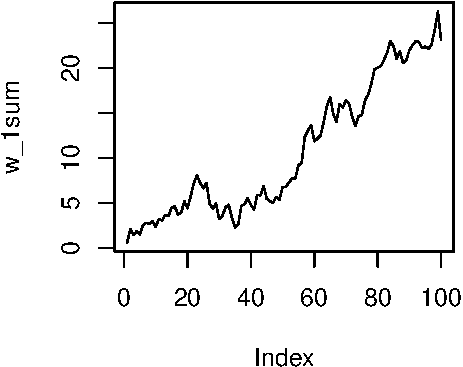
\includegraphics{FMC_T4_PhD_Wiener_Process_files/figure-latex/wiener_process_mean_var-1} \end{center}

\begin{Shaded}
\begin{Highlighting}[]
\CommentTok{# T = 1000}
\NormalTok{T_}\DecValTok{2}\NormalTok{ =}\StringTok{ }\DecValTok{1000}
\NormalTok{w_}\DecValTok{2}\NormalTok{ <-}\StringTok{ }\KeywordTok{rnorm}\NormalTok{(T_}\DecValTok{2}\NormalTok{)}
\NormalTok{w_2sum <-}\StringTok{ }\KeywordTok{cumsum}\NormalTok{(w_}\DecValTok{2}\NormalTok{)}

\KeywordTok{plot}\NormalTok{(w_2sum,}
     \DataTypeTok{type =} \StringTok{"l"}
\NormalTok{     )}
\end{Highlighting}
\end{Shaded}

\begin{center}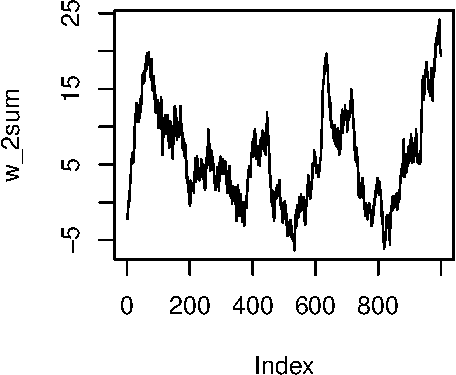
\includegraphics{FMC_T4_PhD_Wiener_Process_files/figure-latex/wiener_process_mean_var-2} \end{center}

\begin{Shaded}
\begin{Highlighting}[]
\CommentTok{# T = 10000}
\NormalTok{T_}\DecValTok{3}\NormalTok{ =}\StringTok{ }\DecValTok{10000}
\NormalTok{w_}\DecValTok{3}\NormalTok{ <-}\StringTok{ }\KeywordTok{rnorm}\NormalTok{(T_}\DecValTok{3}\NormalTok{)}
\NormalTok{w_3sum <-}\StringTok{ }\KeywordTok{cumsum}\NormalTok{(w_}\DecValTok{3}\NormalTok{)}

\KeywordTok{plot}\NormalTok{(w_3sum,}
     \DataTypeTok{type =} \StringTok{"l"}
\NormalTok{     )}
\end{Highlighting}
\end{Shaded}

\begin{center}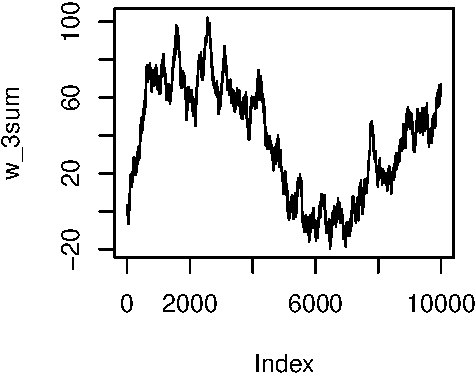
\includegraphics{FMC_T4_PhD_Wiener_Process_files/figure-latex/wiener_process_mean_var-3} \end{center}

While the paths of Wiener Processes are continuous (almost surely) they
are also non-differentiable (almost surely). As a result, we cannot use
our classical ideas of Riemannian integration anymore.

\subsection{Wiener Process with Drift}\label{wiener-process-with-drift}

If the drift rate for a Wiener Process \(X_t\) is \(\mu\) and the
variance change rate is \(\sigma^2\), we can generalize such a process
as: \[dX_t = \mu dt + \sigma dW_t\]

where \(W_t\) is a standard Wiener Process. A discretized version takes
the following form:

\[X_t-X_0 = \mu t+\sigma \epsilon \sqrt{t}\]

which yields \(\mathbb{E}(X_t-X_0)=\mu t\) and
\(\text{var}(X_t-X_0) = \sigma^2 t\). More generally, the drift and
volatility could depend on \(X_t\) in which case we get the classic Ito
Process:

\[X_t-X_0 = \mu(X_t, t) dt+ \sigma(X_t, t)dW_t\]

\section{Ito's Lemma}\label{itos-lemma}

Consider some function \(G(x_1, x_2)\). From calculus we know that:

\[\delta G = \frac{\partial G}{\partial x_1}\cdot \delta x_1 +
\frac{\partial G}{\partial x_2}\cdot \delta x_2 + 
\frac{1}{2!}\frac{\partial^2 G}{\partial x_1^2}\cdot (\delta x_1)^2 +
\frac{1}{2!}\frac{\partial^2 G}{\partial x_2^2}\cdot (\delta x_2)^2 +
\frac{\partial^2 G}{\partial x_1 \partial x_2}\cdot (\delta x_1)(\delta x_2) + \hdots
\]

As \(\delta x_1, \delta x_2\to 0\)

\[dG = \frac{\partial G}{\partial x_1}dx_1 + \frac{\partial G}{\partial x_2}dx_2\]

Now let us suppose that \(G\) depends on \(X_t\) and \(t\) where \(X_t\)
is some Ito Process.

\[\delta G = \frac{\partial G}{\partial x_1}\cdot \delta x_1 +
\frac{\partial G}{\partial t}\cdot \delta t + 
\frac{1}{2!}\frac{\partial^2 G}{\partial x_1^2}\cdot (\delta x_1)^2 +
\frac{1}{2!}\frac{\partial^2 G}{\partial t^2}\cdot (\delta t)^2 +
\frac{\partial^2 G}{\partial x_1 \partial t}\cdot (\delta x_1)(\delta t) + \hdots
\]

A discretized Ito Process is:

\[\delta x = \mu \delta t+\sigma\epsilon \sqrt{t}\]

This may be used to compute \((\delta x)^2\).

\[(\delta x)^2 = \mu^2(\delta t)^2 + \sigma^2 \epsilon^2\delta t+
2\mu\sigma\epsilon(\delta t)^{3/2}=\sigma^2\epsilon^2\delta t+H(\delta t)\]

where \(H(\cdot)\) denote higher order terms in \(\delta t\).

It's clearly seen here that the \((\delta x)^2\) term depends on order
\(\delta t\)

\section*{References}\label{references}
\addcontentsline{toc}{section}{References}

\hypertarget{refs}{}
\hypertarget{ref-Jondeau_Poon_Rockinger:2007}{}
Jondeau, Eric, Ser-Huang Poon, and Michael Rockinger. 2007.
\emph{Financial Modeling Under Non-Gaussian Distributions}. Springer
Finance.

\hypertarget{ref-Tsay:2010}{}
Tsay, Ruey S. 2010. \emph{Analysis of Financial Time Series}. Third
Edition. John Wiley; Sons.


\end{document}
